\documentclass[11pt,a4paper]{article}
\usepackage[T1]{fontenc}
\usepackage[utf8]{inputenc}
\usepackage{lmodern}
\usepackage{textcomp}
\usepackage[left=1.8cm,right=1.8cm,top=3.0cm,bottom=2.2cm,headheight=36pt,headsep=12pt]{geometry}
\usepackage{multicol}
\usepackage{xcolor}
\usepackage{fancyhdr}\usepackage{tikz}
\usepackage{graphicx}
\usepackage{array}
\usepackage{amsmath,amssymb}
\usepackage{setspace}
\usepackage{longtable}
\graphicspath{{../}}
\definecolor{ygreen}{RGB}{46,139,87}\definecolor{dgreen}{RGB}{28,90,56}
\renewcommand{\normalsize}{\fontsize{10.9}{13.4}\selectfont}
\renewcommand{\familydefault}{\rmdefault}
\setlength{\parindent}{0pt}
\setlength{\columnsep}{0.8cm}
\setlength{\columnseprule}{0.4pt}
\setlength{\multicolsep}{3pt plus 1pt minus 1pt}
\renewcommand{\textsubscript}[1]{\ensuremath{_{\text{\fontsize{8}{8}\selectfont #1}}}}
\renewcommand{\textsuperscript}[1]{\ensuremath{^{\text{\fontsize{8}{8}\selectfont #1}}}}
\newcommand{\qn}[1]{\textbf{\fontsize{11.5}{13}\selectfont #1}}
\newcommand{\qsep}{\par\vspace{13pt}}
\newcommand{\fwrule}{\par\vspace{5pt}\noindent\rule{\linewidth}{1.4pt}\par\vspace{7pt}}
\newsavebox{\fitb}
\newcommand{\fitbox}[1]{\sbox{\fitb}{#1}\ifdim\wd\fitb>\linewidth\resizebox{\linewidth}{!}{\usebox{\fitb}}\else\usebox{\fitb}\fi}
\newcommand{\diqqat}[1]{\par\smallskip\noindent\textbf{Diqqat!} #1\par\medskip}
\newcommand{\javob}{\par\nopagebreak[4]\smallskip\noindent\textbf{Javob:} \rule[-2pt]{7.5cm}{0.4pt}\par\smallskip\noindent\textbf{Diqqat!} Javobingizni javoblar varaqasiga ko`chirib yozing.\par\medskip}
\pagestyle{fancy}
\fancyhf{}
\renewcommand{\headrulewidth}{1.6pt}\renewcommand{\headrule}{{\color{ygreen}\hrule height 1.6pt width\headwidth}}
\newcommand{\hdrlogo}{
\begin{tikzpicture}[baseline=0pt]\fill[ygreen,rounded corners=3pt] (0,0) rectangle (0.95,0.95);\node[white,font=\fontsize{24}{26}\bfseries\selectfont] at (0.475,0.47){K};\node[anchor=west,font=\fontsize{16}{18}\bfseries\selectfont,text=dgreen] at (1.15,0.66){KIMYO};\node[anchor=west,font=\footnotesize\scshape,text=gray] at (1.15,0.2){Milliy sertifikat\ \ 2026};\end{tikzpicture}}
\newcommand{\hdrpill}[1]{\begin{tikzpicture}[baseline=0pt]\node[fill=ygreen,text=white,rounded corners=8pt,inner xsep=10pt,inner ysep=5pt,font=\fontsize{13}{15}\bfseries\selectfont] at (0,0.475){#1};\end{tikzpicture}}
\fancyhead[L]{\hdrlogo}
\fancyhead[R]{\hdrpill{16-variant}}

\fancyfoot[C]{\thepage}
\fancypagestyle{first}{\fancyhf{}\renewcommand{\headrulewidth}{1.6pt}\renewcommand{\headrule}{{\color{ygreen}\hrule height 1.6pt width\headwidth}}\fancyhead[L]{\hdrlogo}\fancyhead[R]{\hdrpill{16-variant}}\fancyfoot[C]{\thepage}}
\begin{document}
\normalsize
\thispagestyle{first}
\noindent\textit{Davriy jadvaldan foydalanish mumkin.}
\par\smallskip
\begin{multicols}{2}
\noindent\qn{1.} HC$\equiv$C--CH=CH\textsubscript{2} molekulasida sp gibridlangan uglerod atomlari nechta?

\noindent A)~\textsl{3} \hfill B)~\textsl{2} \hfill C)~\textsl{4} \hfill D)~\textsl{1}\par
\qsep
\noindent\qn{2.} K\textsubscript{2}MnO\textsubscript{4} tarkibida Mn ning oksidlanish \textbf{darajasini aniqlang.}

\noindent A)~\textsl{+1} \hfill B)~\textsl{$-$3} \hfill C)~\textsl{+7} \hfill D)~\textsl{+6}\par
\qsep
\noindent\qn{3.} 0,2 M HCl eritmasining normal \textbf{konsentratsiyasini (n) aniqlang.}

\noindent A)~\textsl{0,4} \hfill B)~\textsl{0,1} \hfill C)~\textsl{0,2} \hfill D)~\textsl{0,3}\par
\qsep
\noindent\qn{4.} Quyidagi tuz eritmalari aralashtirilganda qaysilarida faqat cho`kma hosil bo`ladi? 1) CaCl\textsubscript{2} va Na\textsubscript{2}CO\textsubscript{3}; 2) Na\textsubscript{2}CO\textsubscript{3} va HCl; 3) Al\textsubscript{2}(SO\textsubscript{4})\textsubscript{3} va Na\textsubscript{2}S; 4) Al\textsubscript{2}(SO\textsubscript{4})\textsubscript{3} va Na\textsubscript{2}CO\textsubscript{3}

\noindent A)~\textsl{3} \hfill B)~\textsl{2, 4} \hfill C)~\textsl{1} \hfill D)~\textsl{2, 3}\par
\qsep
\noindent\qn{5.} ZnSO\textsubscript{4} ning suvli eritmasi inert elektrodlar bilan elektroliz qilinganda qaysi moddalar ajraladi?

\noindent\begin{tabular}{@{}p{0.47\linewidth}@{}p{0.47\linewidth}@{}}
A)~\textsl{Zn, H\textsubscript{2} va O\textsubscript{2}} & B)~\textsl{H\textsubscript{2}, Cl\textsubscript{2} va NaOH} \\
C)~\textsl{H\textsubscript{2} va O\textsubscript{2}} & D)~\textsl{Ag va O\textsubscript{2}} \\
\end{tabular}\par
\qsep
\noindent\qn{6.} CO va CH\textsubscript{4} aralashmasi tarkibida CO ning mol miqdori aralashmadagi umumiy mol miqdorining 3/8 qismini tashkil etadi. Aralashmaning massasi 16,4 g. Aralashmaning vodorodga nisbatan \textbf{zichligini aniqlang.}

\noindent A)~\textsl{20,5} \hfill B)~\textsl{5,12} \hfill C)~\textsl{10,25} \hfill D)~\textsl{14}\par
\qsep
\noindent\qn{7.} A + B $\to$ mahsulot reaksiyada v = k$\cdot$[A]\textsuperscript{1}$\cdot$[B]\textsuperscript{1}. Idish hajmi 3 marta kamaytirilsa (T = const), reaksiya tezligi necha marta o`zgaradi?

\noindent A)~\textsl{3} \hfill B)~\textsl{27} \hfill C)~\textsl{9} \hfill D)~\textsl{18}\par
\qsep
\noindent\qn{8.} Na\textsubscript{2}CO\textsubscript{3} va CaCO\textsubscript{3} aralashmasi (62,4 g) mo`l xlorid kislota bilan ta'sirlashganda 13,44 l (n.sh.) gaz ajraldi. Sarflangan HCl \textbf{massasini (g) hisoblang.}

\noindent A)~\textsl{43,8} \hfill B)~\textsl{21,9} \hfill C)~\textsl{87,6} \hfill D)~\textsl{29,2}\par
\qsep
\noindent\qn{9.} N\textsubscript{2}O\textsubscript{4} $\rightleftarrows$ 2NO\textsubscript{2} reaksiyasi 5 l hajmli idishda o`tkazildi. Ma'lumotlar jadvalda berilgan:
\begin{center}
\renewcommand{\arraystretch}{1.15}
\fitbox{\begin{tabular}{|c|c|c|}\hline
\textbf{Modda} & \textbf{N\textsubscript{2}O\textsubscript{4}} & \textbf{NO\textsubscript{2}} \\ \hline
Boshlang`ich, mol & 3 & 0 \\ \hline
Muvozanatda, mol & --- & 4 \\ \hline
\end{tabular}}
\end{center}
Muvozanat \textbf{konstantasini (K) hisoblang.}

\noindent A)~\textsl{6,4} \hfill B)~\textsl{1,6} \hfill C)~\textsl{16} \hfill D)~\textsl{3,2}\par
\qsep
\noindent\qn{10.} 2NO + O\textsubscript{2} $\to$ 2NO\textsubscript{2} reaksiyasida (v = k$\cdot$[NO]\textsuperscript{2}$\cdot$[O\textsubscript{2}]) harorat 40 \textdegree{}C ga oshirildi ($\gamma$ = 3), shu bilan birga NO konsentratsiyasi 3 marta kamaytirildi. Reaksiya tezligi qanday o`zgaradi (necha marta ortadi/kamayadi)? Tezlikning yangi/eski \textbf{nisbatini toping.}

\noindent A)~\textsl{18} \hfill B)~\textsl{4,5} \hfill C)~\textsl{81} \hfill D)~\textsl{9}\par
\qsep
\noindent\qn{11.} Cu + HNO\textsubscript{3} $\to$ Cu(NO\textsubscript{3})\textsubscript{2} + NO + H\textsubscript{2}O reaksiyasida 3 mol Cu erisa, HNO\textsubscript{3} ning necha moli oksidlovchi vazifasini bajaradi?

\noindent A)~\textsl{8} \hfill B)~\textsl{6} \hfill C)~\textsl{2} \hfill D)~\textsl{4}\par
\qsep
\noindent\qn{12.} PCl\textsubscript{5} $\rightleftarrows$ PCl\textsubscript{3} + Cl\textsubscript{2} reaksiyasi 4 l hajmli idishda o`tkazildi. Ma'lumotlar jadvalda berilgan:
\begin{center}
\renewcommand{\arraystretch}{1.15}
\fitbox{\begin{tabular}{|c|c|c|}\hline
\textbf{Modda} & \textbf{PCl\textsubscript{5}} & \textbf{PCl\textsubscript{3}} \\ \hline
Boshlang`ich, mol & 4 & 0 \\ \hline
Muvozanatda, mol & --- & 1 \\ \hline
\end{tabular}}
\end{center}
PCl\textsubscript{5} ning necha foizi reaksiyaga \textbf{kirishganini aniqlang.}

\noindent A)~\textsl{12,5} \hfill B)~\textsl{37,5} \hfill C)~\textsl{75} \hfill D)~\textsl{25}\par
\qsep
\noindent\qn{13.} CuSO\textsubscript{4}$\cdot$5H\textsubscript{2}O kristallogidrat namunasi (50 g) bosqichma-bosqich qizdirilganda uning massasi o`zgarishi grafikda keltirilgan.
\begin{center}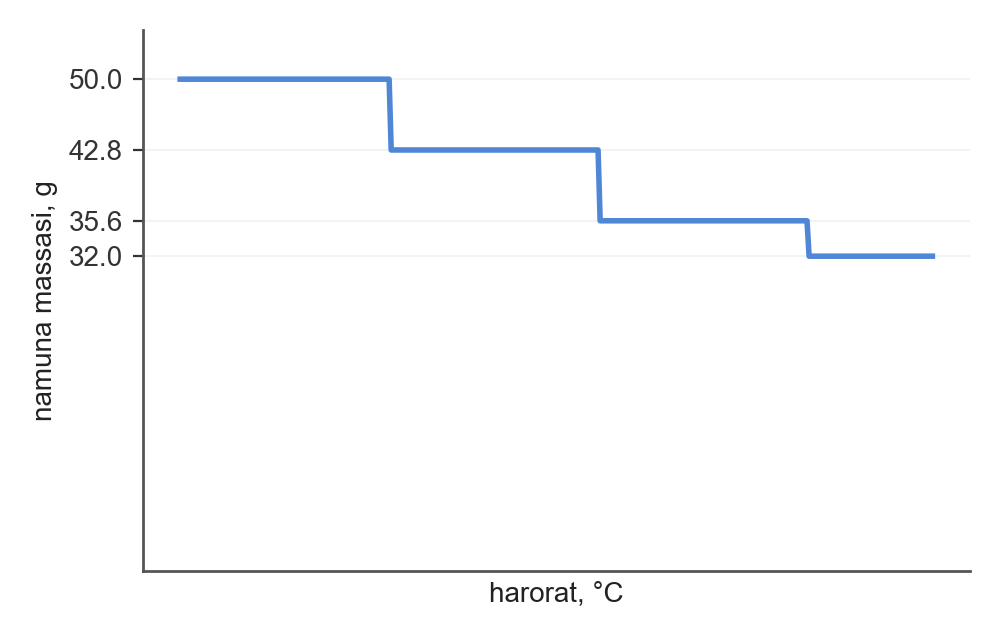
\includegraphics[width=0.86\linewidth]{rasmlar/gen/hy_v16_0.png}\end{center}
Qizdirish natijasida ajralgan suvning umumiy \textbf{massasini (g) hisoblang.}

\noindent A)~\textsl{32} \hfill B)~\textsl{50} \hfill C)~\textsl{18} \hfill D)~\textsl{36}\par
\qsep
\noindent\qn{14.} Rasmdagi o`zgarishlar zanjirida \textit{X} moddaning \textbf{formulasini aniqlang.}
\begin{center}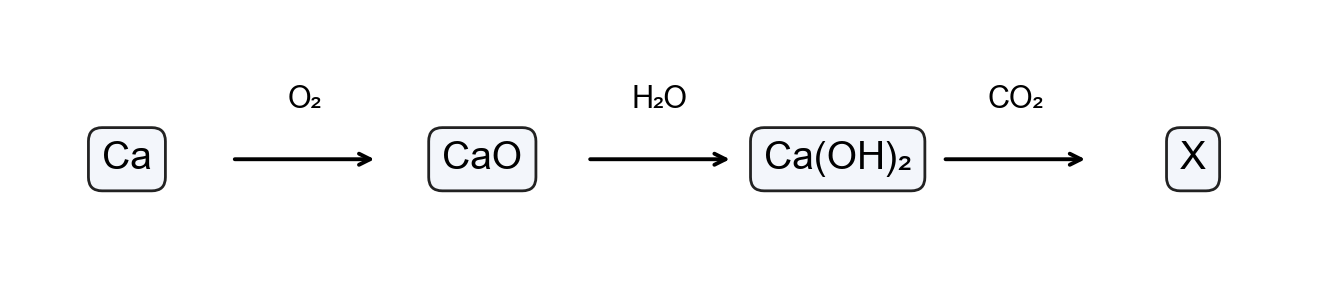
\includegraphics[width=0.86\linewidth]{rasmlar/gen/ci_509279.png}\end{center}

\noindent A)~\textsl{CaO} \hfill B)~\textsl{SO\textsubscript{3}} \hfill C)~\textsl{Ca(OH)\textsubscript{2}} \hfill D)~\textsl{CaCO\textsubscript{3}}\par
\qsep
\noindent\qn{15.} P $\to$ ? $\to$ ? $\to$ ? o`zgarishlar zanjirida (reagentlar: O\textsubscript{2}, H\textsubscript{2}O, KOH) 1-bosqichda hosil bo`ladigan modda \textbf{formulasini toping.}

\noindent A)~\textsl{P\textsubscript{2}O\textsubscript{5}} \hfill B)~\textsl{NaOH} \hfill C)~\textsl{CuSO\textsubscript{4}} \hfill D)~\textsl{SO\textsubscript{2}}\par
\qsep
\noindent\qn{16.} 34 g AgNO\textsubscript{3} to`liq parchalanguncha qizdirildi. Qattiq qoldiq \textbf{massasini (g) aniqlang.}

\noindent A)~\textsl{34} \hfill B)~\textsl{43,2} \hfill C)~\textsl{10,8} \hfill D)~\textsl{21,6}\par
\qsep
\noindent\qn{17.} Qaysi juftliklar o`zaro reaksiyaga kirishmaydi? 1) MgCl\textsubscript{2} va KNO\textsubscript{3}; 2) NaCl va HNO\textsubscript{3}; 3) Fe va HNO\textsubscript{3}(sovuq kons.); 4) CuSO\textsubscript{4} va NaOH

\noindent A)~\textsl{1, 3, 4} \hfill B)~\textsl{1, 2, 3} \hfill C)~\textsl{1, 2} \hfill D)~\textsl{2, 3}\par
\qsep
\noindent\qn{18.} 68 g ammiak katalitik oksidlanib NO ga (unum 80\%), so`ng NO\textsubscript{2} va HNO\textsubscript{3} gacha (umumiy unum 75\%) aylantirildi. Barcha reaksiyalar 2 atm bosimda olib borildi. Hosil bo`lgan nitrat kislota \textbf{massasini (g) hisoblang.}

\noindent A)~\textsl{252} \hfill B)~\textsl{302,4} \hfill C)~\textsl{201,6} \hfill D)~\textsl{151,2}\par
\qsep
\noindent\qn{19.} Ammofos tarkibida NH\textsubscript{4}H\textsubscript{2}PO\textsubscript{4} va (NH\textsubscript{4})\textsubscript{2}HPO\textsubscript{4} mol nisbati 2 : 1. Shu o`g`itdagi azotning massa \textbf{ulushini (\%) toping.}

\noindent A)~\textsl{11,6} \hfill B)~\textsl{23,2} \hfill C)~\textsl{15,47} \hfill D)~\textsl{30,94}\par
\qsep
\noindent\qn{20.} CH\textsubscript{3}--CH(CH\textsubscript{3})--CH(C\textsubscript{2}H\textsubscript{5})--CH\textsubscript{2}--CH\textsubscript{3} birikmaning sistematik nomi qaysi qatorda to`g`ri keltirilgan?

\noindent\begin{tabular}{@{}p{0.47\linewidth}@{}p{0.47\linewidth}@{}}
A)~\textsl{2-metil-3-etilpentan} & B)~\textsl{3-izopropilpentan} \\
C)~\textsl{2,3-dietilbutan} & D)~\textsl{3-etil-2-metilpentan} \\
\end{tabular}\par
\qsep
\noindent\qn{21.} Karbon kislotalar haqida qaysi fikrlar to`g`ri? 1) Benzoy kislota Na\textsubscript{2}CO\textsubscript{3} bilan reaksiyaga kirishmaydi; 2) Sirka angidrid ikki molekula sirka kislotadan suv chiqib hosil bo`ladi; 3) Qattiq suvda sovun yaxshi ko`piklanadi; 4) Karboksil guruh karbonil va gidroksil guruhlardan iborat

\noindent A)~\textsl{2, 4} \hfill B)~\textsl{1, 3} \hfill C)~\textsl{1, 2} \hfill D)~\textsl{1, 2, 4}\par
\qsep
\noindent\qn{22.} Aminlar, aminokislotalar va oqsillar haqida qaysi fikrlar to`g`ri? 1) Dipeptidda 2 ta peptid bog` bor; 2) Anilin bromli suv bilan oq cho`kma beradi; 3) Aminokislotalar faqat kislotali xossaga ega; 4) Glitsin optik faol

\noindent A)~\textsl{2} \hfill B)~\textsl{2, 3} \hfill C)~\textsl{4} \hfill D)~\textsl{2, 4}\par
\qsep
\noindent\qn{23.} 78 g benzol nitrolandi (unum 90\%), hosil bo`lgan nitrobenzol Zinin reaksiyasi bo`yicha qaytarildi (unum 50\%). Barcha reaksiyalar 1 atm bosimda olib borildi. Olingan anilin \textbf{massasini (g) hisoblang.}

\noindent A)~\textsl{83,7} \hfill B)~\textsl{41,9} \hfill C)~\textsl{20,9} \hfill D)~\textsl{93}\par
\qsep
\noindent\qn{24.} Formaldegid va etanal aralashmasi (12,6 g) mo`l ammiakli kumush oksid eritmasi bilan qizdirilganda 118,8 g kumush ajraldi. Qizdirish 15 daqiqa davom etdi. Aralashmadagi etanalning \textbf{massasini (g) aniqlang.}

\noindent A)~\textsl{6} \hfill B)~\textsl{6,6} \hfill C)~\textsl{13,2} \hfill D)~\textsl{6,3}\par
\qsep
\noindent\qn{25.} 324 g kraxmal gidrolizlanib (unum 75\%) glukoza olindi, glukoza esa spirtli bijg`ishga uchradi (unum 60\%). Hosil bo`lgan etanol \textbf{massasini (g) toping.}

\noindent A)~\textsl{41,4} \hfill B)~\textsl{82,8} \hfill C)~\textsl{165,6} \hfill D)~\textsl{138}\par
\qsep
\noindent\qn{26.} Propan qizdirilib, quyidagi sxema bo`yicha parchalandi: C\textsubscript{3}H\textsubscript{8} $\to$ C\textsubscript{3}H\textsubscript{6} + H\textsubscript{2}. Qizdirish 20 daqiqa davom etdi. Hosil bo`lgan gazlar aralashmasining vodorodga nisbatan zichligi 11 bo`lsa, propanning parchalanish \textbf{unumini (\%) aniqlang.}

\noindent A)~\textsl{50} \hfill B)~\textsl{100} \hfill C)~\textsl{80} \hfill D)~\textsl{200}\par
\qsep
\noindent\qn{27.} 22,4 l (n.sh.) CH\textsubscript{4} dan quyidagi sxema bo`yicha etilen olindi: CH\textsubscript{4} $\to$ CH\textsubscript{3}Cl $\to$ C\textsubscript{2}H\textsubscript{6} $\to$ C\textsubscript{2}H\textsubscript{4}. Bosqichlarning unumi ketma-ket 40\%, 85\%, 50\% ni tashkil qiladi. Olingan etilen \textbf{massasini (g) aniqlang.}

\noindent A)~\textsl{4,76} \hfill B)~\textsl{1,19} \hfill C)~\textsl{2,38} \hfill D)~\textsl{28}\par
\qsep
\noindent\qn{28.} 39 g C\textsubscript{6}H\textsubscript{6} dan quyidagi sxema bo`yicha polistirol olindi: C\textsubscript{6}H\textsubscript{6} $\to$ C\textsubscript{6}H\textsubscript{5}--C\textsubscript{2}H\textsubscript{5} $\to$ C\textsubscript{6}H\textsubscript{5}--CH=CH\textsubscript{2} $\to$ (--CH\textsubscript{2}--CH(C\textsubscript{6}H\textsubscript{5})--)n. Bosqichlarning unumi ketma-ket 60\%, 60\%, 75\% ni tashkil qiladi. Barcha reaksiyalar 2 atm bosimda olib borildi. Olingan polistirol \textbf{massasini (g) aniqlang.}

\noindent A)~\textsl{28,08} \hfill B)~\textsl{14,04} \hfill C)~\textsl{7,02} \hfill D)~\textsl{18,72}\par
\qsep
\noindent\qn{29.} 184 g C\textsubscript{6}H\textsubscript{5}CH\textsubscript{3} dan quyidagi sxema bo`yicha 120 g etilbenzoat olindi: C\textsubscript{6}H\textsubscript{5}CH\textsubscript{3} $\to$ C\textsubscript{6}H\textsubscript{5}COOH $\to$ C\textsubscript{6}H\textsubscript{5}COOC\textsubscript{2}H\textsubscript{5}. Dastlabki 1 bosqichning unumi ketma-ket 80\% ga teng. Oxirgi bosqichning \textbf{unumini (\%) aniqlang.}

\noindent A)~\textsl{25} \hfill B)~\textsl{50} \hfill C)~\textsl{40} \hfill D)~\textsl{100}\par
\qsep
\noindent\qn{30.} Natriy xlorid, natriy bromid va natriy yodid eritmalarini (moddalarini) bir-biridan qaysi reagent yordamida farqlash mumkin?

\noindent\begin{tabular}{@{}p{0.47\linewidth}@{}p{0.47\linewidth}@{}}
A)~\textsl{kumush nitrat} & B)~\textsl{xlorid kislota} \\
C)~\textsl{natriy gidroksid} & D)~\textsl{bariy xlorid} \\
\end{tabular}\par
\qsep
\noindent\qn{31.} Quyidagi aralashmani ajratish uchun qaysi usul mos: temir qipig`i va oltingugurt kukuni?
\noindent A)~\textsl{magnit yordamida ajratish (temir tortiladi)}\par
\noindent B)~\textsl{bug`latish}\par
\noindent C)~\textsl{ajratgich voronka}\par
\noindent D)~\textsl{distillash (fraksiyalab haydash)}\par
\qsep
\noindent\qn{32.} Rasmda spirt lampasi alangasi ko`rsatilgan. Probirkani qizdirishda alanganing qaysi qismidan foydalaniladi?
\begin{center}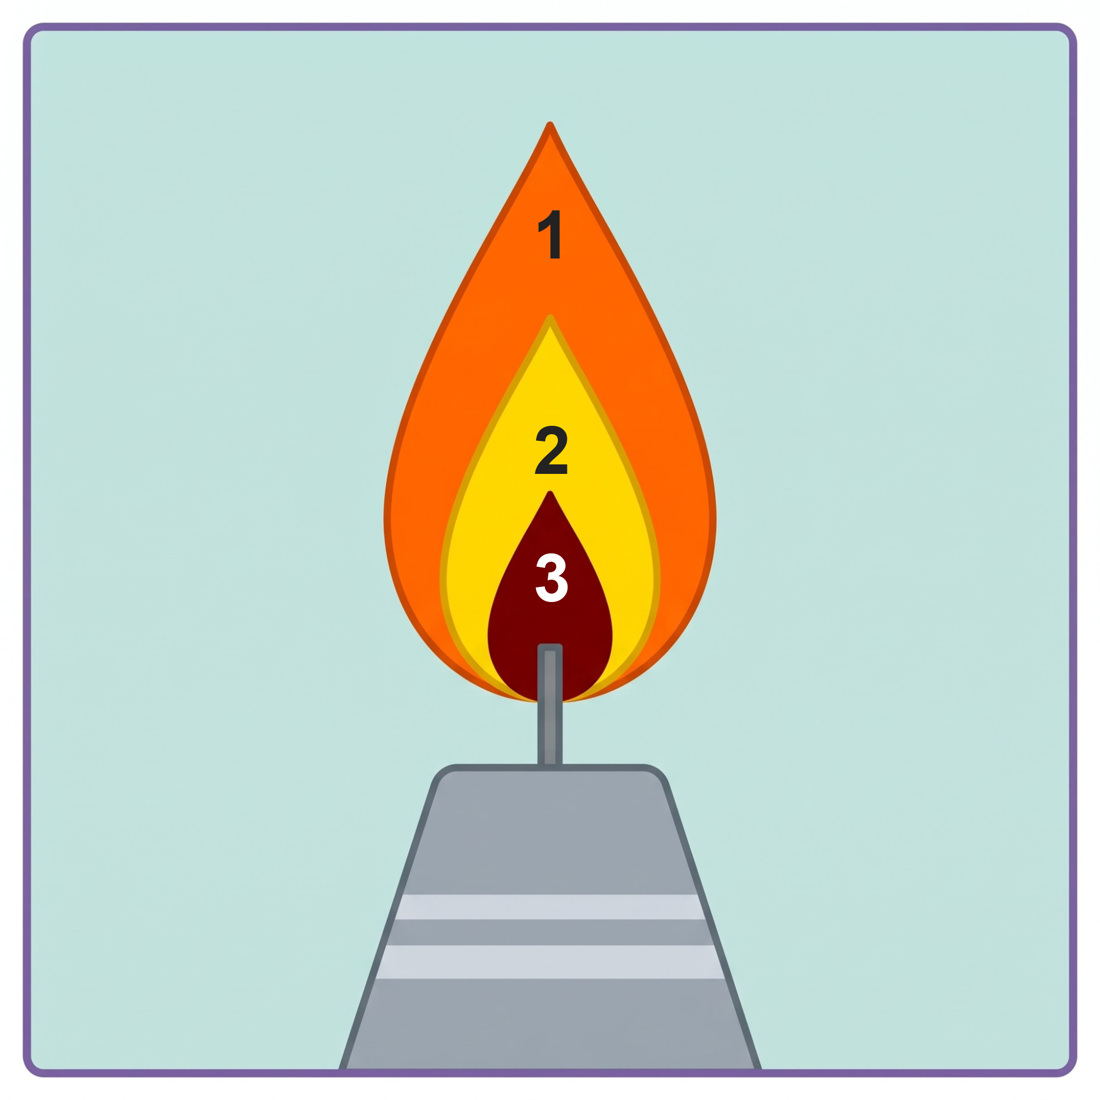
\includegraphics[width=0.86\linewidth]{rasmlar/darslik/d_alanga.png}\end{center}
\noindent A)~\textsl{1 -- yuqori chetki xira qism}\par
\noindent B)~\textsl{3 -- pastki qism, pilikka yaqin}\par
\noindent C)~\textsl{hamma qismidan bir xil}\par
\noindent D)~\textsl{2 -- o`rta ravshan qism   ---}\par
\qsep
\end{multicols}
\medskip
\noindent\setlength{\fboxsep}{0pt}\fbox{\begin{tabular}{p{0.74\linewidth}|p{0.2\linewidth}}
\parbox[t]{0.72\linewidth}{\vspace{3pt}\textbf{Topshiriqlar (33--35) va javob variant (A--F)larini o`zaro to`g`ri moslashtiring.} 18,8 g Cu(NO\textsubscript{3})\textsubscript{2} doimiy massagacha qizdirildi, ajralgan gazlar suvga yuttirilib, hajmi 2 l bo`lgan eritma tayyorlandi. Qoldiq shu eritmada to`liq eritildi (kislota qoldiqsiz sarflandi), olingan eritma (hajmi o`zgarmadi deb hisoblang) 10 A tok kuchi bilan 1544 s inert elektrodlarda elektroliz qilindi.
\vspace{3pt}} & \parbox[t]{0.19\linewidth}{\vspace{3pt}A~\textsl{4,1}\\[3pt]
B~\textsl{1}\\[3pt]
C~\textsl{10,24}\\[3pt]
D~\textsl{5,12}\\[3pt]
E~\textsl{0,05}\\[3pt]
F~\textsl{0,03}}\\ \hline
\parbox[t]{0.72\linewidth}{\vspace{2pt}\textbf{33. Gazlar yutilgach hosil bo`lgan eritmaning pH ini aniqlang.}\vspace{2pt}} & \\ \hline
\parbox[t]{0.72\linewidth}{\vspace{2pt}\textbf{34. Qoldiq erigandan so`ng Cu(NO\textsubscript{3})\textsubscript{2} ning molyar konsentratsiyasini (mol/l) hisoblang.}\vspace{2pt}} & \\ \hline
\parbox[t]{0.72\linewidth}{\vspace{2pt}\textbf{35. Elektrolizda katodda ajralgan metall massasini (g) toping.}\vspace{2pt}} & 
\end{tabular}}
\par\bigskip
\noindent\qn{36.} NaCrO\textsubscript{2} + Br\textsubscript{2} + NaOH $\to$ Na\textsubscript{2}CrO\textsubscript{4} + NaBr + H\textsubscript{2}O reaksiya tenglamasini tenglang va barcha koeffitsiyentlar \textbf{yig`indisini aniqlang.}
\javob\qsep
\noindent\qn{37.} 300 g 10\% li CuSO\textsubscript{4} eritmasiga m g CuSO\textsubscript{4}$\cdot$5H\textsubscript{2}O eritildi, natijada tuzning massa ulushi 20,8\% ga yetdi. m \textbf{ni (g) toping.}
\javob\qsep
\noindent\qn{38.} Oksidlanish darajasi +3 bo`lgan noma'lum \textit{X} metallning xloridi 31,7 g massada mo`l AgNO\textsubscript{3} eritmasi bilan ta'sirlashganda 86,1 g cho`kma hosil bo`ldi. Reagent (AgNO\textsubscript{3}) eritmasining massa ulushi 50\% va zichligi 1,18 g/ml; u mo`l miqdorda olingan. \textit{X} metallning nisbiy atom \textbf{massasini toping.}
\javob\qsep
\noindent\qn{39.} Uglevodorodning 5,8 g massasi yondirilganda 17,6 g CO\textsubscript{2} va 9 g H\textsubscript{2}O hosil bo`ldi. Tajriba 10 daqiqa davom etdi. Uglevodorod molekulasidagi uglerod atomlari \textbf{sonini toping} (M = 58 g/mol).
\javob\qsep
\noindent\qn{40.} 44,5 g tristearin mo`l NaOH eritmasi bilan to`liq gidrolizlandi (sovun unumi 80\%). Barcha reaksiyalar 2 atm bosimda olib borildi. Hosil bo`lgan natriy stearat (M = 306 g/mol) \textbf{massasini (g) toping.}
\javob\qsep
\par\bigskip\begin{center}\textbf{\fontsize{13}{15}\selectfont YOZMA ISH}\end{center}
\noindent\qn{41.} \textbf{Topshiriqni bajarish jarayonida barcha reaksiya tenglamalarini yozing. Miqdoriy va arifmetik hisoblashlarni (unga asos bo`lgan usul yoki formulani ko`rsatgan holda) uzviy ketma-ketlikda bajaring.}\par\smallskip
\textit{X} -- oksidlanish darajasi +2 bo`lgan metall. \textit{X}(NO\textsubscript{3})\textsubscript{2} tuzining 66,2 g namunasi doimiy massagacha qizdirilganda hosil bo`lgan qattiq qoldiq massasi tuz massasining 67,4\% ini tashkil etdi. Ajralgan gazlar aralashmasi sovitilib, 200 g suvga to`liq yuttirildi; so`ngra qattiq qoldiq hosil bo`lgan eritmada to`liq eritildi (kislota qoldiqsiz sarflandi). Olingan eritma inert elektrodlar yordamida 10 A tok kuchi bilan 1930 s elektroliz qilindi (\textit{X} ning bir qismi eritmada qoldi).\par
\noindent 1)\ Barcha jarayonlarning reaksiya tenglamalarini yozing va tenglashtiring; qoldiq massa ulushidan foydalanib, \textit{X} metallni aniqlang.\par
\noindent 2)\ Qizdirishda ajralgan gazlar tarkibini (mol) toping va ularni suvga yuttirishdan hosil bo`lgan HNO\textsubscript{3} massasini (g) hisoblang.\par
\noindent 3)\ Qoldiq erigandan keyingi eritmada \textit{X}(NO\textsubscript{3})\textsubscript{2} ning massa ulushini (\%) hisoblang. Natijani dastlabki tuz massasi va suv massasi orqali tushuntiring.\par
\noindent 4)\ Elektrolizda katodda ajralgan metall massasini (g) va anodda ajralgan gaz hajmini (l, n.sh.) toping.\par
\noindent 5)\ Elektroliz tugagach eritmadagi \textit{X}(NO\textsubscript{3})\textsubscript{2} va HNO\textsubscript{3} ning massa ulushlarini (\%) aniqlang.\par
\diqqat{Mazkur topshiriq kengaytirilgan javobni talab etib, uning yechilish usuli va shu usul asosidagi barcha hisoblash amallari javoblar varaqasida aks etishi lozim.}\qsep
\noindent\qn{42.} Quyidagi o`zgarishlar zanjirida \textit{X}, \textit{Y}, \textit{Z} noma'lum organik moddalar:\par
\[\setlength{\fboxsep}{0pt}\text{C\textsubscript{2}H\textsubscript{5}Cl}\xrightarrow{\text{KOH (spirtli)}}\text{\textit{X}}\xrightarrow{\text{H\textsubscript{2}O, H\textsuperscript{+}}}\text{\textit{Y}}\xrightarrow{\text{CuO, t\textdegree{}}}\text{\textit{Z}}\xrightarrow{\text{Ag\textsubscript{2}O, NH\textsubscript{3}}}\text{CH\textsubscript{3}COOH}\]
\noindent 1)\ C\textsubscript{2}H\textsubscript{5}Cl $\to$ \textit{X} : reaksiya tenglamasini yozing; hosil bo`lgan moddani nomlang.\par
\noindent 2)\ \textit{X} $\to$ \textit{Y} : reaksiya tenglamasini yozing; hosil bo`lgan moddani nomlang.\par
\noindent 3)\ \textit{Y} $\to$ \textit{Z} : reaksiya tenglamasini yozing; hosil bo`lgan moddani nomlang.\par
\noindent 4)\ \textit{Z} $\to$ CH\textsubscript{3}COOH : reaksiya tenglamasini yozing; hosil bo`lgan moddani nomlang.\par
\diqqat{Mazkur topshiriq kengaytirilgan javobni talab etib, uning yechilish usuli va shu usul asosidagi barcha hisoblash amallari javoblar varaqasida aks etishi lozim.}\qsep
\noindent\qn{43.} \textbf{Topshiriqni bajarish jarayonida barcha reaksiya tenglamalarini yozing. Miqdoriy va arifmetik hisoblashlarni (unga asos bo`lgan usul yoki formulani ko`rsatgan holda) uzviy ketma-ketlikda bajaring.}\par\smallskip
Alyuminiy kukuni va noma'lum M\textsubscript{2}O\textsubscript{3} oksidi aralashmasi (jami 46,6 g) qizdirilganda reaksiya oxirigacha bordi (M --- oksidlanish darajasi +3 bo`lgan metall, M ning oksidlanish darajasi xlorid kislotada +2 ga o`tadi). Hosil bo`lgan qattiq mahsulot mo`l NaOH eritmasi bilan ishlanganda 6,72 l (n.sh.) gaz ajraldi; erimay qolgan qoldiq esa mo`l xlorid kislota bilan 8,96 l (n.sh.) gaz ajratdi. Aralashmaning zichligi 2,3 g/sm\textsuperscript{3} ga teng. Natriy tetragidroksoalyuminat saqlagan eritmadan mo`l CO\textsubscript{2} o`tkazildi, hosil bo`lgan cho`kma qizdirilib, qoldiq Na\textsubscript{2}CO\textsubscript{3} bilan suyuqlantirildi.\par
\noindent 1)\ Termit jarayoni, mahsulotning NaOH va HCl bilan reaksiyalarini yozing va tenglashtiring.\par
\noindent 2)\ Aralashmadagi alyuminiyning umumiy miqdorini (mol) va ortib qolgan alyuminiy miqdorini hisoblang.\par
\noindent 3)\ Noma'lum M metallni aniqlang. Eritmadan CO\textsubscript{2} o`tkazilganda hosil bo`lgan cho`kma massasini (g) toping.\par
\noindent 4)\ Reaksiyada hosil bo`lgan Al\textsubscript{2}O\textsubscript{3} massasini (g) toping. Cho`kma qizdirilganda hosil bo`lgan oksid massasini (g) hisoblang.\par
\noindent 5)\ Mahsulotdagi ortiqcha alyuminiy va Al\textsubscript{2}O\textsubscript{3} ni to`liq eritish uchun zichligi 1,22 g/ml bo`lgan 20\% li NaOH eritmasidan necha ml kerak? Oksid Na\textsubscript{2}CO\textsubscript{3} bilan suyuqlantirilganda ajralgan gaz hajmini (l, n.sh.) aniqlang.\par
\diqqat{Mazkur topshiriq kengaytirilgan javobni talab etib, uning yechilish usuli va shu usul asosidagi barcha hisoblash amallari javoblar varaqasida aks etishi lozim.}\qsep
\newpage
\noindent\textbf{\fontsize{13}{15}\selectfont 16-variant}\hfill \textbf{Javoblar kaliti}\par\smallskip\hrule\smallskip
\textit{Faqat o`qituvchi uchun.}\par\medskip
\noindent\textbf{1--32-savollar}\par\smallskip
\noindent\begin{tabular}{|c|c|c|c|c|c|c|c|c|c|c|c|c|c|c|c|}\hline
\textbf{1} & \textbf{2} & \textbf{3} & \textbf{4} & \textbf{5} & \textbf{6} & \textbf{7} & \textbf{8} & \textbf{9} & \textbf{10} & \textbf{11} & \textbf{12} & \textbf{13} & \textbf{14} & \textbf{15} & \textbf{16}\\\hline
\textsl{B} & \textsl{D} & \textsl{C} & \textsl{C} & \textsl{A} & \textsl{C} & \textsl{C} & \textsl{A} & \textsl{D} & \textsl{D} & \textsl{C} & \textsl{D} & \textsl{C} & \textsl{D} & \textsl{A} & \textsl{D}\\\hline
\textbf{17} & \textbf{18} & \textbf{19} & \textbf{20} & \textbf{21} & \textbf{22} & \textbf{23} & \textbf{24} & \textbf{25} & \textbf{26} & \textbf{27} & \textbf{28} & \textbf{29} & \textbf{30} & \textbf{31} & \textbf{32}\\\hline
\textsl{B} & \textsl{D} & \textsl{C} & \textsl{D} & \textsl{A} & \textsl{A} & \textsl{B} & \textsl{B} & \textsl{B} & \textsl{B} & \textsl{C} & \textsl{B} & \textsl{B} & \textsl{A} & \textsl{A} & \textsl{A}\\\hline
\end{tabular}\par\medskip
\noindent\textbf{33--35-savollar}\par\smallskip
\noindent\begin{tabular}{|c|c|c|}\hline \textbf{No} & \textbf{Javob} & \textbf{Qiymat}\\\hline
33 & \textsl{B} & 1\\\hline
34 & \textsl{E} & 0,05\\\hline
35 & \textsl{D} & 5,12\\\hline
\end{tabular}\par\medskip
\noindent\textbf{36--40-savollar}\par\smallskip
\noindent\begin{tabular}{|c|c|}\hline \textbf{No} & \textbf{To`g`ri javob}\\\hline
36 & 25\\\hline
37 & 75\\\hline
38 & 52\\\hline
39 & 4\\\hline
40 & 36,72\\\hline
\end{tabular}\par\medskip
\noindent\textbf{41--43-topshiriqlar: javoblar}\par\smallskip
\noindent\textbf{41-topshiriq.}\par
\noindent 1) 207 $\to$ Pb\par
\noindent 2) 25,2 g\par
\noindent 3) 24,87\%\par
\noindent 4) 20,7 g; 1,12 l\par
\noindent 5) 13,57\%; 5,17\%\par
\noindent\textbf{42-topshiriq.}\par
\noindent 1) C\textsubscript{2}H\textsubscript{5}Cl + KOH (spirtli) $\to$ C\textsubscript{2}H\textsubscript{4} (etilen)\par
\noindent 2) C\textsubscript{2}H\textsubscript{4} + H\textsubscript{2}O, H\textsuperscript{+} $\to$ C\textsubscript{2}H\textsubscript{5}OH (etanol)\par
\noindent 3) C\textsubscript{2}H\textsubscript{5}OH + CuO, t\textdegree{} $\to$ CH\textsubscript{3}CHO (sirka aldegid (etanal))\par
\noindent 4) CH\textsubscript{3}CHO + Ag\textsubscript{2}O, NH\textsubscript{3} $\to$ CH\textsubscript{3}COOH (sirka kislota)\par
\noindent\textbf{43-topshiriq.}\par
\noindent 1) 2Al + M\textsubscript{2}O\textsubscript{3} $\to$ Al\textsubscript{2}O\textsubscript{3} + 2M; 2Al + 2NaOH + 6H\textsubscript{2}O $\to$ 2Na[Al(OH)\textsubscript{4}] + 3H\textsubscript{2}$\uparrow$ (Al\textsubscript{2}O\textsubscript{3} ham NaOH da eriydi, gaz bermaydi); M + 2HCl $\to$ M\par
\noindent 2) 0,2 mol; 0,6 mol\par
\noindent 3) Cr; 46,8 g\par
\noindent 4) 20,4 g; 30,6 g\par
\noindent 5) 98,4 ml; 6,72 l\par
\par\bigskip\noindent\textbf{Mavzular taqsimoti}\par\smallskip
{\small\noindent\begin{longtable}{|c|p{7.2cm}|p{5.4cm}|c|}\hline \textbf{No} & \textbf{Mavzu} & \textbf{Tekshiriladigan ko`nikma} & \textbf{Ball}\\\hline
1 & 10-sinf \S{}17 & Bilim va tushunish & 1\\\hline
2 & 8-sinf; Tirkashev \textit{V} bob (oksidlanish darajasi) & Bilim va tushunish & 1\\\hline
3 & 11-sinf 4-bob (normal konsentratsiya) & Hisoblash va masala yechish & 1\\\hline
4 & 9-sinf; 10-sinf (tuzlar gidrolizi, ion almashinish reaksiyalari) & Bilim va tushunish & 1\\\hline
5 & 11-sinf 8-bob; Tirkashev \textit{V} bob (elektroliz) & Bilim va tushunish & 1\\\hline
6 & 8-9-sinf (gaz aralashmalari; Avogadro qonuni) & Hisoblash va masala yechish & 1\\\hline
7 & Tirkashev VI bob (massalar ta'siri qonuni) & Hisoblash va masala yechish & 1\\\hline
8 & 8-9-sinf (karbonatlar; kislotalar bilan reaksiya) & Hisoblash va masala yechish & 1\\\hline
9 & Tirkashev VI bob (muvozanat, jadval) & Jadval tahlili & 1\\\hline
10 & 9-sinf; 11-sinf (reaksiya tezligi; Vant-Goff, massalar ta'siri) & Hisoblash va masala yechish & 1\\\hline
11 & Tirkashev \textit{V} bob; Tashev (HNO\textsubscript{3}, H\textsubscript{2}SO\textsubscript{4}) & Hisoblash va masala yechish & 1\\\hline
12 & Tirkashev VI bob (muvozanat, jadval) & Jadval tahlili & 1\\\hline
13 & 7-sinf (kristallogidratlar) & Grafik tahlili & 1\\\hline
14 & 9-sinf (genetik bog`lanish) & Rasm bo`yicha tahlil & 1\\\hline
15 & 8-sinf; 9-sinf (genetik bog`lanish) & Bilim va tushunish & 1\\\hline
16 & Tashev (nitratlar termik parchalanishi) & Hisoblash va masala yechish & 1\\\hline
17 & 9-sinf; Tashev (anorganik birikmalar xossalari) & Bilim va tushunish & 1\\\hline
18 & 9-sinf (azotning birikmalari; ammiak va HNO\textsubscript{3} olinishi) & Hisoblash va masala yechish & 1\\\hline
19 & 9-sinf (mineral o`g`itlar) & Hisoblash va masala yechish & 1\\\hline
20 & 10-sinf (nomenklatura \S{}6, \S{}11, \S{}20, \S{}24--26) & Bilim va tushunish & 1\\\hline
21 & 10-sinf (mavzuga oid paragraflar); Abdusamatov & Bilim va tushunish & 1\\\hline
22 & 10-sinf (mavzuga oid paragraflar); Abdusamatov & Bilim va tushunish & 1\\\hline
23 & 10-sinf (arenlar, anilin olinishi) & Hisoblash va masala yechish & 1\\\hline
24 & 10-sinf (aldegidlarning kumush ko`zgu reaksiyasi) & Hisoblash va masala yechish & 1\\\hline
25 & 10-sinf (uglevodlar: kraxmal, glukoza) & Hisoblash va masala yechish & 1\\\hline
26 & 10-sinf (alkanlarning krekingi va degidrogenlanishi) & Hisoblash va masala yechish & 1\\\hline
27 & 10-sinf (alkanlar; Vyurs reaksiyasi; degidrogenlash) & Hisoblash va masala yechish & 1\\\hline
28 & 10-sinf (arenlar, polimerlar) & Hisoblash va masala yechish & 1\\\hline
29 & 10-sinf (arenlar, karbon kislotalar, murakkab efirlar) & Hisoblash va masala yechish & 1\\\hline
30 & 9-sinf; 10-sinf (sifat reaksiyalari; moddalarni farqlash) & Bilim va tushunish & 1\\\hline
31 & 7-sinf (aralashmalarni ajratish usullari) & Bilim va tushunish & 1\\\hline
32 & 7-sinf (spirt lampasi alangasi, 5-rasm) & Rasm bo`yicha tahlil & 1\\\hline
33--35 & Aralash masala (moslashtirish) & Ko`p bosqichli hisob & 3\\\hline
36--40 & Qisqa javobli masalalar & Hisoblash & 5\\\hline
41--43 & Yozma ish & Usul va hisob (M, A) & 75\\\hline
\end{longtable}}
\end{document}
